\begin{CJK}{UTF8}{gkai}
\chapter{图像处理}
\end{CJK}


\begin{CJK}{UTF8}{gbsn}


本章中的所有算法都涉及对图像或像素的二维数组执行的操作。通常,图形程序员可能想要更改图像的大小、颜色或其他功能。前三个算法描述了在各种环境下拉伸或缩放图像的技术。第一条强调速度,而第二条强调质量。第四个算法描述了一种使用简化的颜色集显示全彩色图像的方法。


在某些情况下,将多个图像的特征组合起来是很有用的。第七个算法将我们现在熟悉的图像组合代数应用于黑白位图或1位图像。第八个算法讨论了如何有选择地模糊两幅图像,同时结合它们,以模拟相机的光圈景深效果。


有时,期望的结果不是另一个图像,而是图像中某些特征的另一种表示。第五、第六和第九算法描述了从图像中提取区域边界信息的技术。


\newpage
\section{位图快速拉伸}
\begin{center}
\small{
Tomas M\"oller\\
Lund Institute of Technology 
Hoganas, Sweden}
\end{center}

\subsection*{介绍}

这里提出了一个整数算法,用于将位图的任意水平线或垂直线拉伸到任何其他任意直线上。该算法可用于要求接近实时性或实时性的绘图和绘图程序。应用程序区域的例子包括扩大和缩小位图的矩形区域,以及将矩形区域包装到圆形区域上。
\subsection*{算法}
程序本身非常简单,大多数计算机图形程序员可能都熟悉它所基于的Bresenham划线算法(1965)。事实上,它可以基于任何画线算法;然而,Bresenham被选中,因为它是基于整数的,并且在计算机图形社区中非常普遍。对于那些不熟悉Bresenham算法的人来说,伪代码用于在第一个八边形中绘制线段。

\IncMargin{1em}
\begin{algorithm} 
\SetKwData{Left}{left}
\SetKwData{This}{this}
\SetKwData{Up}{up} 
\SetKwFunction{Union}{Union}
\SetKwFunction{WritePixel}{WritePixel}
\SetKwFunction{FindCompress}{FindCompress} 
\SetKwInOut{Input}{input}
\SetKwInOut{Output}{output}

\SetKwData{EdgeSet}{EdgeSet}
\SetKwData{Point}{point}
	
	\Input{由点(x1,y1)和点(x2,y2)构成的线段} 
	\Output{将线段绘制到位图上}
	 \BlankLine 
	 \BlankLine
	 
	 
	 
	 \tcp{从(x1, y1)到(x2, y2)在第一个八边形内画一条线;
所有变量都是整数}
	dx $\leftarrow$ x2 - x1\\
	dy $\leftarrow$ y2 - y1\\
	e $\leftarrow$ 2 * dy - dx\\
	\For{i$\leftarrow$ 1,i$\leqslant$ dx, i$\leftarrow$ i+1}{
		\WritePixel(x1,y1)	\tcp{在图上显示(x1,y1)}
		\While{e$\geqslant$ 0}{
			y1 $\leftarrow$ y1 + 1\\
			e $\leftarrow$ e - 2 * dx\\
		}
		x1 $\leftarrow$ x1 + 1\\
		e $\leftarrow$ e + 2 * dy
	}
	 
	 
	 
 	 	  \caption{Line(x1,y1,x2,y2)}
 	 	  \label{algo:Line} 
 	 \end{algorithm}
\DecMargin{1em} 

上面的伪代码也适用于第二个八分位数,但是在这种情况下,行不会是连续的,因为x1总是递增1。这非常适合算法。


让我们回到拉伸算法的解释上。x1和y1不能被解释为二维直线上的一对坐标,它们必须被解释为一维坐标。dx必须解释为目标线的长度,dy是源线的长度。使用这些解释,x1是目标线上的坐标,y1是源线上的坐标。对于目标线上的每个像素,从源线上选择一个像素。这些像素以统一的方式选择。参见图\ref{fig:drawline}。
\begin{figure}[htbp]%[htbp]
  \centering
  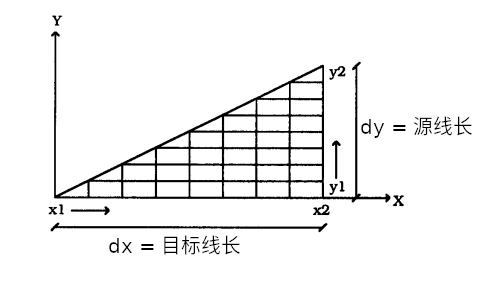
\includegraphics[totalheight=2in]{./fig/1.png}
  \caption{源线与目标线} 
  \label{fig:drawline}
\end{figure}

如果$dx$大于$dy$,那么目标线比源线长。因此,在绘制到目的线上时,源线将被放大。另一方面,如果$dy$大于$dx$,源线就会减小。如果$dx = dy$,算法会得到与源相同的直线。下面是伪代码中完整的stretcher算法,重写后能够处理$x2 < x1$和$y2 < y1$的行。

\IncMargin{1em}
\begin{algorithm} 
\SetKwData{Left}{left}
\SetKwData{This}{this}
\SetKwData{Up}{up} 
\SetKwFunction{Union}{Union}
\SetKwFunction{WritePixel}{WritePixel}
\SetKwFunction{Abs}{abs}
\SetKwFunction{Sign}{sign}
\SetKwFunction{ReadPixel}{ReadPixel}
\SetKwFunction{SetColor}{SetColor}
\SetKwFunction{FindCompress}{FindCompress} 
\SetKwInOut{Input}{input}
\SetKwInOut{Output}{output}

\SetKwData{EdgeSet}{EdgeSet}
\SetKwData{Point}{point}
	
	\Input{} 
	\Output{}
	 \BlankLine 
	 \BlankLine
	 
	 
	 
	 \tcp{从(x1, y1)到(x2, y2)在第一个八边形内画一条线;
所有变量都是整数}
	\tcp{将源线(y1 ~ y2)延伸到目标线(x1 ~ x2)。}
	\tcp{源线和目标线都是水平的}
	\tcp{yr =从其中读取像素的水平线}
	\tcp{yw =要写入像素的水平线}
	\tcp{ReadPixel(x, y)返回像素(x, y)处的颜色}
	\tcp{WritePixel(x, y) 用当前颜色写入(x, y)处的像素}
	\tcp{SetColor(Color) 设置当前写入的颜色为Color}
	dx $\leftarrow$ \Abs(x2 - x1)\\
	dy $\leftarrow$ \Abs(y2 - y1)\\
	sx $\leftarrow$ \Sign(x2 - x1)\\
	sy $\leftarrow$ \Sign(y2 - y1)\\
	e $\leftarrow$ 2 * dy - dx\\
	dx2 $\leftarrow$ 2 * dx\\
	dy $\leftarrow$ 2 * dy\\
	\For{i$\leftarrow$ 1,i$\leqslant$ dx, i$\leftarrow$ i+1}{
		color $\leftarrow$ \ReadPixel(x, y)\\
		\SetColor(Color)\\
		WritePixel(x1, yw)
		
		\While{e$\geqslant$ 0}{
			y1 $\leftarrow$ y1 + sy\\
			e $\leftarrow$ e - dx2\\
		}
		x1 $\leftarrow$ x1 + 1\\
		e $\leftarrow$ e + 2 * dy
	}
	 
	 
	 
 	 	  \caption{Stretch(x1, y1, x2, y2, yr, yw)}
 	 	  \label{algo:Stretch} 
 	 \end{algorithm}
\DecMargin{1em} 

如果$x$等于0,那么符号函数不需要返回0,因为$dx$或$dy$都等于0,这意味着一条长度为1的直线。由于该算法只使用整数运算,而不使用乘法或除法,因此非常高效和快速。


这个小程序的另一个有趣之处是,它可以用来生成几种不同形状的位图。下面列出了一些可以用来渲染的东西。
\subsection*{一些项目使用位图扩展器}
\begin{itemize}
	\item 包裹在圆形或椭圆形区域上的矩形图片。关于绕圈,请参阅附录中的源代码。
	\item 放大和缩小位图的矩形部分。参见附录中的源代码。
	\item 将位图的矩形部分绕平行梯形包绕。例如,一个绕x或y轴旋转,然后进行透视转换的矩形可以用作目标形状。
\end{itemize}


\subsection*{进一步的工作}
为了改进算法,也许可以添加一个抗锯齿例程.\\
See also G1, 147; G1, 166; G3, A.2.




\newpage
\section{一般的滤波图像缩放}
\begin{center}
\small{
Dale Schumacher\\
St. Paul, Minnesota}
\end{center}


栅格图像可以看作是连续二维函数$f(x, y)$的样本的矩形网格。这些样本被假定为连续函数在给定样本点的精确值。理想的光栅图像缩放程序包括重建原始的连续函数,然后以不同的速率重新采样该函数(Pratt, 1991;Foley $ et al$., 1990 )。采样率越高(采样越靠近),采样就越多,图像也就越大。采样率越低(采样间隔越远)产生的样本越少,因此图像越小。幸运的是,我们不需要真正地重建整个连续函数,而只是确定重建函数在与新样本对应的点上的值,这是一个更容易的任务(Smith, 1981)。仔细选择过滤器,这个重采样过程可以分两步进行,首先水平地拉伸或缩小图像,然后垂直地拉伸或缩小(反之亦然),可能有不同的比例因子。双通道方法的运行时成本$O$(image\_width*image\_height* (filter\_width + filter\_height)比简单的二维过滤$O$(image\_width*image\_height*filter\_width*filter\_height)要低得多。

\begin{figure}[htbp]%[htbp]
  \centering
  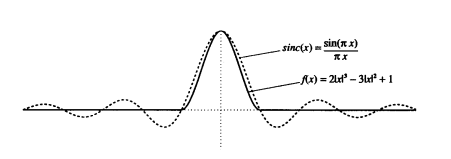
\includegraphics[totalheight=1.7in]{./fig/1.2.1.png}
  \caption{$sinc$示例} 
  \label{fig:sinc}
\end{figure}

放大图像的过程有很多名字,包括放大、拉伸、缩放、插值和上采样。我将把这个过程称为放大。缩小图像的过程也有很多名字,包括缩小、缩小、按比例缩小、抽取和下采样。我将把这个过程称为简化。这些过程将在一维而不是二维中进行解释,因为缩放是在每个轴上独立进行的。

在放大过程中,我们通过应用滤波函数来确定每个源像素对每个目标像素的贡献。采样理论表明,$sinc$函数$f(x) = \sin(πx)/πx$是理想的重构函数;然而,我们有一个有限的样本集,并且需要一个具有有限支持的过滤器(即过滤器非零的区域)。我在这个例子中使用的过滤器是一个三次函数,$f(x) = 2|x| 3 - 3|x| 2 +1$,从- 1到+1,当单独应用时,它覆盖了每个样本的单位体积。图1比较了这些过滤函数。重采样滤波器的设计是一个没完没了的争论的来源,超出了这个宝石的范围,但在许多其他作品中讨论(Pratt, 1991; Turkowski, 1990; Mitchell, 1988; Smith, 1982; Oppenheim and Schafer, 1975; Rabiner and Gold, 1975).。为了应用滤镜,我们将滤镜函数的副本放在每个源像素的中心,并缩放到该像素的高度。对于每个目标像素,我们计算源图像中相应的位置。我们将这一点上加权滤波函数的值相加,以确定目标像素的值。图\ref{fig:sinc2}说明了这个过程。

\begin{figure}[htbp]%[htbp]
  \centering
  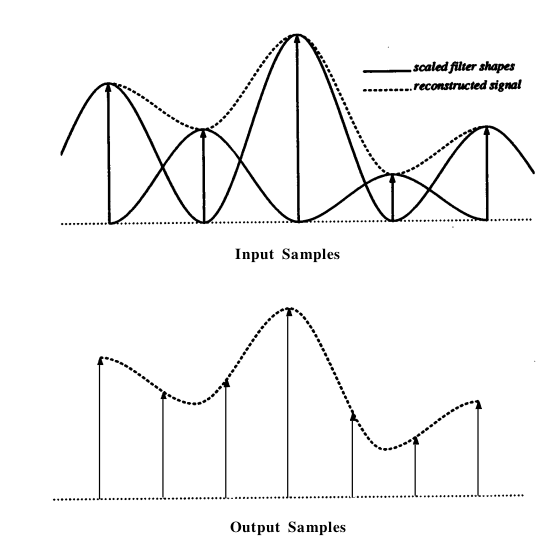
\includegraphics[totalheight=4in]{./fig/1.2.2.png}
  \caption{滤波示例} 
  \label{fig:sinc2}
\end{figure}

在缩小过程中,过程是相似的,但不完全相同,因为我们必须考虑频率混叠。采样理论将奈奎斯特频率定义为能够正确捕获连续源信号中所有频率成分的采样率。奈奎斯特频率是源信号中最高频率分量频率的两倍。任何频率成分高于采样率的一半将被不正确地采样,并将被混叠到一个更低的频率。

因此,重构信号将只包含采样率的一半或更少的频率成分。在放大过程中,我们拉伸重构信号,降低其分量频率。然而,在缩小过程中,我们正在缩小重构信号,提高其分量频率,并可能超过我们新的采样率的奈奎斯特频率。为了创建合适的样本,我们必须消除重采样奈奎斯特频率以上的所有频率成分。这可以通过图像缩小因子拉伸滤波函数来实现。此外,由于每个源像素处的滤波器更宽,和将按比例更大,并应除以相同的因子进行补偿。图\ref{fig:sinc3}说明了这个过程。

\begin{figure}[htbp]%[htbp]
  \centering
  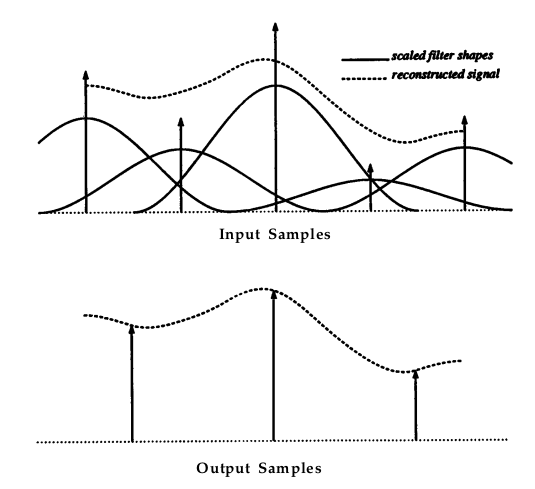
\includegraphics[totalheight=4in]{./fig/1.2.3.png}
  \caption{滤波示例} 
  \label{fig:sinc3}
\end{figure}

到目前为止,我们只考虑了一维情况。我们将其扩展到典型的光栅图像的二维情况,首先水平缩放,然后垂直缩放。这里将不再演示缩放最小目标轴的进一步优化。滤波操作会导致大量的计算,所以我们尽可能多地预先计算。每个行(或列)的缩放过程是相同的。过滤器的位置和面积是固定的;这样,我们就可以预先计算出每个目标像素的贡献者和相应的滤波器权值。计算目标像素贡献者的伪代码如\ref{algo:calculate_contributions}。

\IncMargin{1em}
\begin{algorithm} 
\SetKwData{Left}{left}
\SetKwData{This}{this}
\SetKwData{Up}{up} 
\SetKwFunction{Union}{Union}
\SetKwFunction{WritePixel}{WritePixel}
\SetKwFunction{Abs}{abs}
\SetKwFunction{Floor}{floor}
\SetKwFunction{Ceiling}{ceiling}
\SetKwFunction{Sign}{sign}
\SetKwFunction{ReadPixel}{ReadPixel}
\SetKwFunction{SetColor}{SetColor}
\SetKwFunction{FindCompress}{FindCompress} 
\SetKwFunction{Filter}{filter}
\SetKwFunction{AddContributor}{add\_contributor}

\SetKwInOut{Input}{input}
\SetKwInOut{Output}{output}

\SetKwData{EdgeSet}{EdgeSet}
\SetKwData{Point}{point}
	
	\Input{} 
	\Output{}
	 \BlankLine 
	 \BlankLine
	 
	 
	 
	 %\tcp{从(x1, y1)到(x2, y2)在第一个八边形内画一条线;所有变量都是整数}
	
	scale $\leftarrow$ dst\_size/src\_size;\\
	center $\leftarrow$ destination/scale;\\
	\If{scale < 1.0}{
		width $\leftarrow$ filter\_width/scale;\\
		fscale $\leftarrow$ 1.0/scale;\\
	}
	\lElse{
		width $\leftarrow$ filter\_width;\\
		fscale $\leftarrow$ 1.0;\\	
	}
	left $\leftarrow$ \Floor(center - width);\\
	right $\leftarrow$ \Ceiling(center + width);\\
	\For{source $\leftarrow$ left,source $\leftarrow$ source + 1, source $\leqslant$ right}{
		weight ← \Filter((center – source)/fscale)/fscale;
		\AddContributor(destination, source, weight);
	}
	 
	 
	 
 	 	  \caption{calculate\_contributions(destination)}
 	 	  \label{algo:calculate_contributions} 
 	 \end{algorithm}
\DecMargin{1em} 

在计算出贡献之后,目标图像的所有行(或列)都可以使用相同的预计算的过滤器值进行处理。下面的伪代码\ref{algo:scale_row}显示了这些值用于扩展单个目标行的应用程序。

\IncMargin{1em}
\begin{algorithm} 
\SetKwData{Left}{left}
\SetKwData{This}{this}
\SetKwData{Up}{up} 
\SetKwFunction{Union}{Union}
\SetKwFunction{WritePixel}{WritePixel}
\SetKwFunction{Abs}{abs}
\SetKwFunction{Floor}{floor}
\SetKwFunction{Ceiling}{ceiling}
\SetKwFunction{Sign}{sign}
\SetKwFunction{ReadPixel}{ReadPixel}
\SetKwFunction{SetColor}{SetColor}
\SetKwFunction{FindCompress}{FindCompress} 
\SetKwFunction{Filter}{filter}
\SetKwFunction{AddContributor}{add\_contributor}

\SetKwInOut{Input}{input}
\SetKwInOut{Output}{output}

\SetKwData{EdgeSet}{EdgeSet}
\SetKwData{Point}{point}
	
	\Input{} 
	\Output{}
	 \BlankLine 
	 \BlankLine
	 
	 
	 
	 %\tcp{从(x1, y1)到(x2, y2)在第一个八边形内画一条线;所有变量都是整数}
	
	\For{ i ← 0, i ← i + 1, i < dst\_size }{
		v ← 0;\\
		\For{ j ← 0, j ← j + 1, j < contributors[i] }{
			s ← contributor[i][j];\\
			w ← weight\_value[i][j];\\
			v ← v + (source\_row[s]*w);\\
		}
		destination\_row[i] ← v;\\
	}
	
 	 	  \caption{scale\_row(destination\_row, source\_row)}
 	 	  \label{algo:scale_row} 
 	 \end{algorithm}
\DecMargin{1em} 


\begin{figure}[htbp]%[htbp]
  \centering
  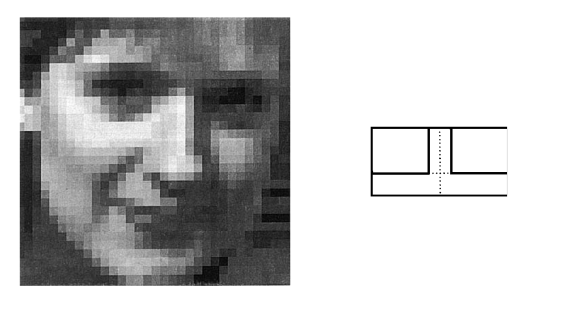
\includegraphics[totalheight=2in]{./fig/1.2.4.png}
  \caption{滤波示例} 
  \label{fig:sinc4}
\end{figure}

\begin{figure}[htbp]%[htbp]
  \centering
  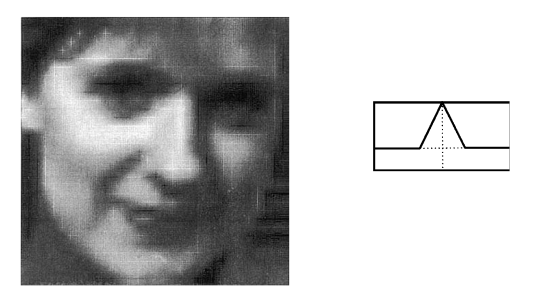
\includegraphics[totalheight=2in]{./fig/1.2.5.png}
  \caption{滤波示例} 
  \label{fig:sinc5}
\end{figure}

\begin{figure}[htbp]%[htbp]
  \centering
  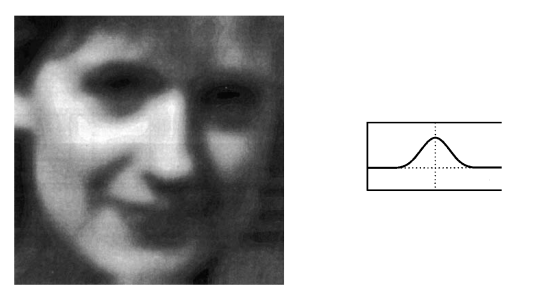
\includegraphics[totalheight=2in]{./fig/1.2.6.png}
  \caption{滤波示例} 
  \label{fig:sinc6}
\end{figure}

\begin{figure}[htbp]%[htbp]
  \centering
  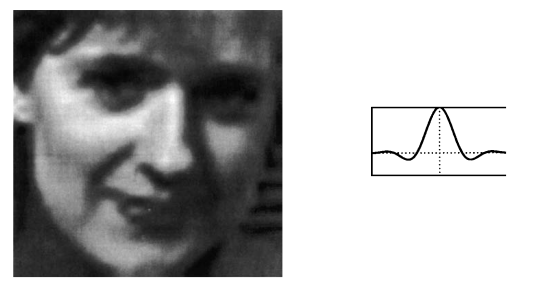
\includegraphics[totalheight=2in]{./fig/1.2.7.png}
  \caption{滤波示例} 
  \label{fig:sinc7}
\end{figure}

\begin{figure}[htbp]%[htbp]
  \centering
  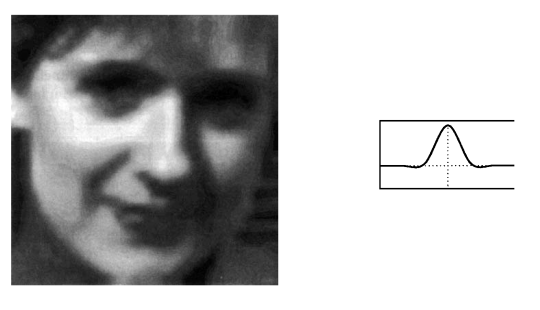
\includegraphics[totalheight=2in]{./fig/1.2.8.png}
  \caption{滤波示例} 
  \label{fig:sinc8}
\end{figure}

然后将相同的过程应用于图像的列—首先根据垂直比例因子(可能与水平比例因子不同)预计算过滤器的贡献,然后处理从中间(水平比例)图像到最终目标图像的列。

在附录中提供的源代码中,给出了许多过滤器函数,可以很容易地添加新的函数。zoom()函数以所需过滤器的名称和过滤器支持作为参数。图\ref{fig:sinc4}到图\ref{fig:sinc8}显示了不同滤波器对样本图像的影响,以及每个滤波器函数的脉冲响应图。

样本图像在两个方向上都按比例放大了12倍。图\ref{fig:sinc4}显示了一个框过滤器,它相当于直接复制像素值,因为它显示了相当多的平铺或“锯齿”。图\ref{fig:sinc5}显示了三角形或Bartlett滤波器,相对于方框来说是一个相当大的改进,计算仍然简单,但仍然有明显的过渡线。图\ref{fig:sinc6}显示了一个三次b样条,它没有产生尖锐的过渡,但是它的宽度导致了过度的模糊。三角形和b样条函数分别通过盒形滤波器与自身卷积1次和3次来计算。图\ref{fig:sinc7}显示了Lanczos 3滤波器,一个在$-3$到$+3$范围外衰减为零的$sinc$函数,它显示了在完全sinc函数时出现的过度的“振铃”效应。图\ref{fig:sinc8}显示了Mitchell滤波器($B = \frac{1}{3}, C =\frac{1}{3} $),一个没有急剧过渡的三次函数,以及“振铃(ringing)”和“模糊(blurring)”效果之间的一个很好的折衷。

See also G1, 147; G1, 166; G3, A.1.

\newpage
\section{位图缩放操作的优化}
\begin{center}
\small{
Dale Schumacher\\
St. Paul Minnesota}
\end{center}

这一节描述了一系列位图缩放操作的优化。我们没有给出一般的缩放算法,而是利用了几个特定于应用程序的限制,这些限制允许显著减少执行时间:每像素图像的位、已知的源和目标位图大小、以及位压缩的水平光栅存储和显示格式。示例应用程序是在典型的视频监视器上显示传真位图图像。

我们首先假设在内存中有源FAX,未压缩,存储为8位字节,每个字节的高阶位表示沿水平行的一组8个字节中最左边的像素。此外,在选择示例缩放因子时,我们假设源FAX的分辨率在两个方向上都是200点每英寸。如果数据是常用的200 × 100 dpi格式,我们可以通过复制每个扫描线使其为200 × 200 dpi,这是我们在解压阶段经常可以处理的任务。最初,我们将假设数据存储为与显示所用的位值匹配的白色和黑色位值。下面将讨论一种反演0位和1位含义的好方法。最后,我们假设目标位图的格式与源位图相同。

由于我们的示例图像分辨率高于您的典型视频监视器,我们将只考虑缩小图像的情况,而不是放大它。同样,我们用8来表示比例因子,$ \frac{7}{8}=87.5\%$,$ \frac{6}{8}=75\%$,$\frac{5}{8}=62.5\%$,$ \frac{4}{8}=50\%$,$ \frac{3}{8}=37.5\%$,$\frac{2}{8}=25\% $。一般算法工作如下:从源图像中取一条扫描线。对于每个字节,使用字节值作为查找表的索引,该查找表给出给定输入字节的简化位。将派生的输出位移位到累加器中。每个输入字节加到累加器的位数是基于比例因子的(例如,如果我们减少到$ \frac{5}{8} $比例,我们为每个8位输入生成5位输出)。当累加器中至少有8位时,我们从累加器中删除最左边的8位,并将它们作为输出字节写入目标扫描行。扫描线末端剩余的任何位都会被移到相应的位置并输出。许多源扫描线可以完全跳过,再次基于比例因子(例如,在$ \frac{5}{8} $的比例下,我们每8个扫描线中只处理5个,跳过3个)。

\begin{figure}[htbp]%[htbp]
  \centering
  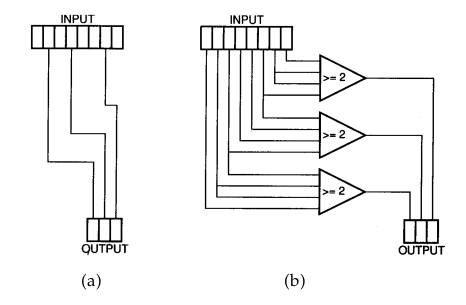
\includegraphics[totalheight=2.3in]{./fig/1.3.1.png}
  \caption{缩放操作} 
  \label{fig:1.3.1}
\end{figure}

既然已经理解了基本的算法,我们可以讨论一些有用的变化和改进过程。该算法的核心是约简查找表。如果我们需要反转最终图像中的黑白图像,一种方法是反转查找表中存储的位。然后,它将映射到1111b,而不是$00000000b$映射到$00000b$。这本质上给了我们在缩放期间免费的光度反演。类似地,通过仔细创建查找表,我们可以解决另一个问题,同样是免费的。如果我们缩小到$\frac{3}{8}$的比例,我们将在每8位中寻找3个来输出。图\ref{fig:1.3.1}a显示了这样做的最简单的方法。一个更好的方法是模拟一种对源比特进行滤波或加权平均的形式,如图\ref{fig:1.3.1}b所示。由于查找表可以在编译时创建,所以使用更复杂的算法创建表的计算成本与运行时性能无关。为了进行适当的过滤缩放,我们真的应该跨相邻扫描线和跨字节边界应用过滤器。由于这些操作会带来很高的运行时成本,并且以有限的方式应用过滤,我们可以在没有额外成本的情况下展示改进,所以我们做的是便宜的事情。即使在这些限制条件下,使用滤波也比直接对输入进行子采样要好,如图\ref{fig:1.3.1}a所示。

您喜欢的任何类型的传递函数都可以以同样的方式应用,在8位跨度的限制内,并且仅以黑白作为输入值。您甚至可以做一些事情,如反转位的顺序,这可以与不同的存储顺序一起使用,以使图像从左到右翻转,或将其旋转180度(以防有人将图像倒过来输入扫描仪)。将表扩展到16位,这将占用128Kb的内存,而不是8位表使用的256b,从而提供了更大的灵活性。使用16位时,您可以使用更大的跨度,并且可以选择16倍而不是8倍的比例因数,这可能会使您的视频显示尺寸更匹配。这些技术以及附录中给出的示例代码只是简单的构建块。检查您自己的应用程序的约束,以找到更多应用这些原则和提高代码性能的方法。

See also G1, 147; G1, 166; G2, 57; G2, 84.



\newpage
\section{一个简单的减色滤镜}
\begin{center}
\small{
Dennis Bragg\\
Graphics Software Inc.\\
Bullard, Texas}
\end{center}
\subsection*{介绍}
提出了一个简单的滤波器,将一个24位的彩色光栅图像减少到15位有效位,并消除了可见的颜色步进问题。所得到的图像可以直接显示在16位帧缓冲器上,或用作颜色量化方法的输入,以进一步减少图像中的颜色数量。

光栅图像通常存储为一个24位像素数组,8位分配给每个红、绿、蓝(RGB)组件。每个RGB组件包含256种可能的强度级别。图1(见彩色插入图)是一个24位图像,使用了2215种不同的颜色。注意彩色球平滑连续的阴影。

不幸的是,能够显示24位彩色图像的帧缓冲区并不总是可用的。使用8位像素作为256色彩色地图索引的彩色显示器被广泛使用。颜色量化方法(Gervautz和Purgathofer, 1990)常用于减少24位图像中使用的颜色数量,以便在8位设备上准确显示。

每像素可以显示16位颜色的帧缓冲器(每个RGB组件5位,加上一个属性位)也变得越来越便宜。在16位帧缓冲区上显示24位图像的典型解决方案是屏蔽每个RGB组件的三个最不重要的位。这种方法将每种颜色的256个强度级别减少到只有32个级别。

一个发生在减色平滑阴影图像的问题是颜色步进。在原始24位图像中,亮度从暗到亮连续变化的区域,在16位或8位帧缓冲区中显示时,通常会出现明显的亮度级步骤。在第2页(见彩色插入图)中,第1页的图像使用Gervautz和Purgathofer的颜色量化方法减少到256色。由于可供选择的颜色数量有限,请注意踏在球上的颜色。

该宝石通过一个加权随机量来改变每个像素RGB组件的强度级别,从而解决了颜色步进问题。方差量的加权方式这种方法的结果图像中任何像素局部区域的平均值非常接近源图像的实际24位颜色。

结果图像每像素包含15个有效的颜色位,每个RGB组件包含5个有效的颜色位。图像可以直接显示在16位帧缓冲区上,或用作颜色量化方法的输入,以进一步减少颜色的数量。得到的图像有一些“颗粒”的外观,但比可见的颜色梯度要少得多。

\subsection*{滤波器}

过滤器分别考虑每个像素的RGB组件。将一个分量的256个强度等级划分为32个相等的区域。每个区域覆盖8个强度等级。第一个区域的强度等级为0,下一个区域的强度等级为8,以此类推。

RGB组件的强度将被设置为这些区域之一。如果将组件设置为最接近的强度级别,得到的图像仍然会显示颜色步进。相反,强度除以8(或模量)的余数被确定。这给出了一个从0到7的数字。生成一个范围为0到8的随机数,并与余数进行比较。如果余数小于或等于随机数,则分量强度增加8。这具有以一种随机的方式改变组件的效果,但偏重于最接近的强度水平。

接下来,根据用户提供的噪声水平,将一些随机噪声添加到组件强度中。噪音的添加消除了任何残留的色彩踏步,否则可能是显而易见的。最后,组件较低的3位被屏蔽,将每像素的有效位数减少到15。

这个过程产生的RGB组件与原始的24位组件有很大的不同。然而,图像任意局部区域的像素分量的平均强度与原始图像的平均强度非常接近。在第三张图中(见彩色插入图),首先对原始的24位图像进行滤波处理,然后采用与图2相同的方法将图像压缩到每像素8位。
\subsection*{实现}
这个过滤器是用函数rgbvary()实现的。该函数需要四个参数:一个由待处理像素的RGB组件组成的三个字符数组(RGB),一个指定所需噪声级别的整数(noise\_level),以及像素的$x$和$y$位置($x$和$y$)。

该函数返回源RGB数组中修改后的RGB组件。噪音等级可以从0(无噪音)到8(吵闹!)2级的噪音在实践中效果很好。

像素的x和y位置由两个宏(jitterx和jittery)使用,它们生成随机数。抖动宏基于GRAPHICS GEMS中的抖动函数(Cychosz, 1990)。使用抖动的优点是它总是在特定的$x$, $y$位置上以相同的幅度变化一个像素。当你在动画中减少几帧的色彩时,这是很重要的。使用标准的随机数生成器将在动画播放时产生“雪花”效果。jitter函数消除了这个问题。

在调用rgbvary()以初始化jitter宏使用的查找表之前,必须调用函数jitter\_init()。这个过程使用标准的C函数rand()来填写表格。

\subsection*{总结}

一种滤波器被提出,以减少24位图像为15有效位每像素。该程序消除了颜色步进的问题,但代价是外观略有颗粒。生成的图像可以直接显示在16位帧缓冲上,或用作颜色量化方法的输入,以进一步减少颜色。

\begin{figure}[htbp]%[htbp]
  \centering
  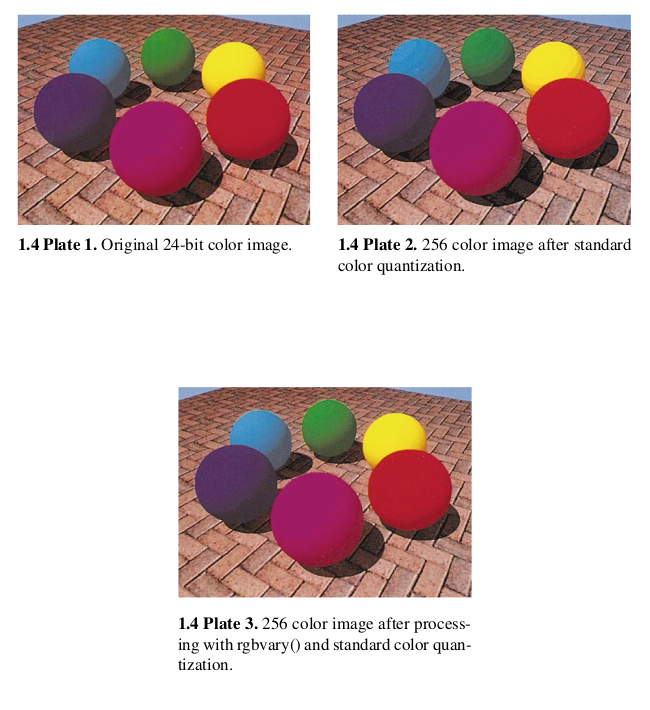
\includegraphics[totalheight=5in]{./fig/1.4.png}
  \caption{颜色滤波} 
  \label{fig:1.4}
\end{figure}

\newpage
\section{从抽样数据得到的紧凑等高线}
\begin{center}
\small{
Dennis Bragg\\
Graphics Software Inc.\\
Bullard, Texas}
\end{center}


\subsection*{问题}
包括医学成像、地震学和气象学在内的许多领域的数据,都是在一个大立方体网格的顶点上采集的一组测量数据。在这些领域中,从数据立方体生成可视化表示的技术非常重要。许多常见的可视化技术将数据值视为连续函数$F$的样本函数值,并对某些$c$生成$F(x, y, z) = c$的分段平面近似,即函数的等值线。最初的《图形瑰宝》之一,“从采样数据定义表面”,调查了几种最著名的从数据立方体生成等高线的技术(Hall, 1990)。

在本文中,我们将对该类型的所有技术进行增强。这种增强减少了任何等高线近似的元素数量,并改善了元素的形状。第一个改进通常将表示的大小减少约$50\%$,允许更快的重新显示并减少内存需求。第二种方法通过避免在许多照明模型中造成不希望看到的阴影影响的狭窄元素,从而得到质量更好的图片。

\subsection*{基于立方体的轮廓}
一些作者提出了大致类似的方法,可以从立方体数据网格中创建可视化的等高线。这些方法分别处理每个立方体上的数据,并利用沿立方体边缘的线性插值来计算位于等高线上的点集合。在Lorenson和Cline的Marching Cubes算法(Lorenson和Cline, 1987)中,这些交点通过表查找来连接成边和三角形,表查找的基础是定义立方体顶点的值$F(x, y, z) - c$的符号。

不幸的是,这种方法并不能保证轮廓的连续性,因为共享一张带有混合符号的脸的相邻立方体可以以不同的方式划分(Durst, 1988)。其他人提出了另一种方法,通过对模糊人脸中心的函数进行采样来消除这种情况的歧义(Wyvil等人,1986)。我们称之为这样的方法,通过沿着三次网格边缘的线性插值计算出轮廓的顶点,基于边缘的插值方法。

基于边缘的插值方法的另一个问题是,它们产生的表面网格可能非常不规则,即使是简单的三元数据。这些不规则性包括微小的三角形(当轮廓通过立方体网格的顶点时产生)和狭窄的三角形(当轮廓通过网格的边缘时产生)。根据我们的经验,在某些曲面网格中,这种三角形可以占到三角形的$50\%$。这些形状糟糕的元素通常会降低渲染算法和有限元分析应用于网格的性能,而对近似的总体精度贡献很小。

\subsection*{紧凑立方体}
这个章节的贡献是一种通用的技术,用于从基于边的插值中消除近简并三角形的问题。该技术背后的想法很简单:当网格的一个顶点靠近表面时,将网格“弯曲”一点,这样顶点就位于表面上。小三角形坍缩成点,小三角形坍缩成边,只剩下形状良好的大三角形。本文的其余部分概述了这一理念的实现;有更详细的解释(Moore和Warren, 1991)。

对数据立方体应用任何基于边的插值算法,并在此过程中,记录沿着立方体边缘生成的每个顶点,该顶点附近的立方体网格的点。我们称这个顶点为它最近的网格点的卫星。如果顶点位于一条边的中点,则可以使用这条边的任意端点,只要共享这条边的所有其他立方体使用同一个端点。当算法的这一阶段完成后,就得到了等高线的三角剖分S和一个离三角剖分的每个顶点最近的网格点。
\begin{figure}[htbp]%[htbp]
  \centering
  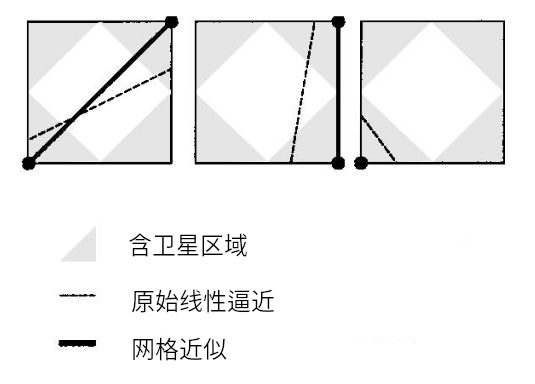
\includegraphics[totalheight=1.8in]{./fig/1.5.1.png}
  \caption{二维案例表紧凑型立方体} 
  \label{fig:1.5.1}
\end{figure}

\begin{figure}[htbp]%[htbp]
  \centering
  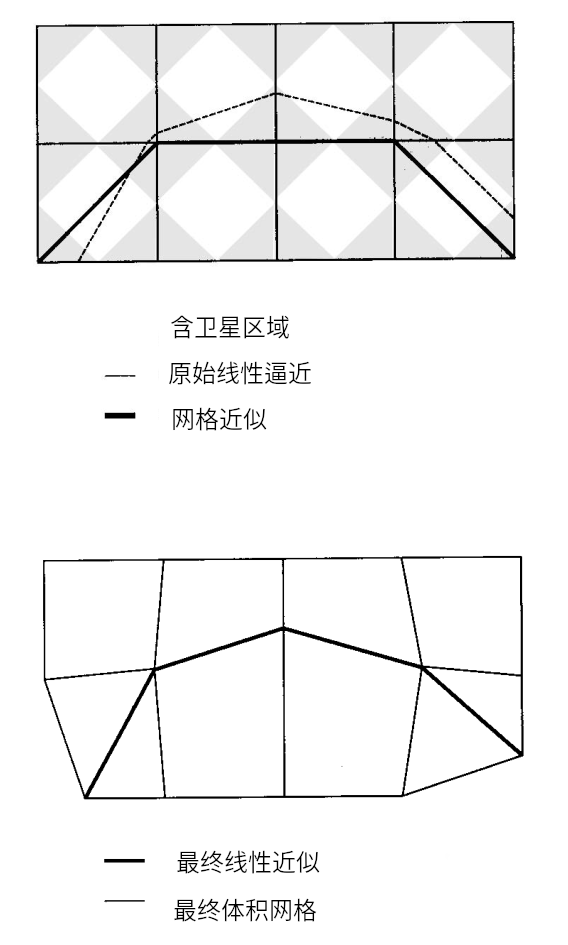
\includegraphics[totalheight=4in]{./fig/1.5.2.png}
  \caption{一个二维立方体的例子} 
  \label{fig:1.5.2}
\end{figure}

为了得到一个新的、更小的等值线近似值,请采用以下步骤:
\IncMargin{1em}
\begin{algorithm} 
\SetKwData{Left}{left}
\SetKwData{This}{this}
\SetKwData{Up}{up} 
\SetKwFunction{Union}{Union}
\SetKwFunction{WritePixel}{WritePixel}
\SetKwFunction{Abs}{abs}
\SetKwFunction{Floor}{floor}
\SetKwFunction{Ceiling}{ceiling}
\SetKwFunction{Sign}{sign}
\SetKwFunction{ReadPixel}{ReadPixel}
\SetKwFunction{SetColor}{SetColor}
\SetKwFunction{FindCompress}{FindCompress} 
\SetKwFunction{Filter}{filter}
\SetKwFunction{AddContributor}{add\_contributor}

\SetKwInOut{Input}{input}
\SetKwInOut{Output}{output}

\SetKwData{EdgeSet}{EdgeSet}
\SetKwData{Point}{point}
	
	%\Input{} 
	%\Output{}
	 \BlankLine 
	 \BlankLine
	 
	 
	 
	 %\tcp{从(x1, y1)到(x2, y2)在第一个八边形内画一条线;所有变量都是整数}
	
	\For{ each triangle $T$ in $S$ }{
		\If{the vertices of $T$ are satellites of distinct gridpoints}{
			produce a triangle connecting the gridpoints\;
		}
		\Else{
			$T$ collapses to a vertex or edge so ignore it\;
		}
		\For{ each gridpoint $g$ of the new triangulation }{
			displace $g$ to the average position of its satellites;
		}
	}
	
 	 	  \caption{等值线近似值}
 	 	  \label{algo:approximation} 
 	 \end{algorithm}
\DecMargin{1em} 










\end{CJK}
